\chapter{Camps magnètics d'espires i bobines}
\begin{resum}
Aquesta pràctica té com a objectiu principal l'estudi dels camps magnètics creats per diferents configuracions d'espires i bobines. Mitjançant una sonda Hall s'han mesurat els camps creats, al seu centre, per espires de radis diferents, així com per conjunts de una, dues i tres espires. De la mateixa manera s'han realitzat mesures del camp magnètic al llarg de l'eix de bobinas de diversos radis.

Amb les dades experimentals s'ha posat a prova la dependència del camp magnètic d'una espira del seu radi i també del nombre d'espires, tal i com prediu la llei de Biot-Savart. També s'ha pogut trobar un valor per a la permeabilitat magnètica del buit, \( \mu_0 \).
\end{resum}

\section{Introducció}
L'objectiu d'aquesta pràctica és mesurar i posteriorment analitzar els camps magnètics que resulten de la circulació de corrent elèctric per fils conductors. Més precisament, es disposarà de diverses espires i bobines per a la circulació del corrent. En el cas de les espires, es mesurarà el camp al centre d'espires de diferents radis i s'analitzarà la variació del camp en funció del radi. Per les bobines el que s'estudiarà és el camp magnètic a diferents punts de l'interior de bobines de diferent nombre de voltes i de diferents radis.

\section{Mètode experimental}
\subsection{Espires}
Pel que fa a les espires, primerament s'ha muntat el circuit que inclou el teslàmetre amb la sonda, l'amperímetre, el regle i l'espira indicada en cada cas. La \cref{fig:circuit teslametre} mostra un esquema d'aquest circuit.

\begin{figure}[htb]
  \centering \small \sffamily
  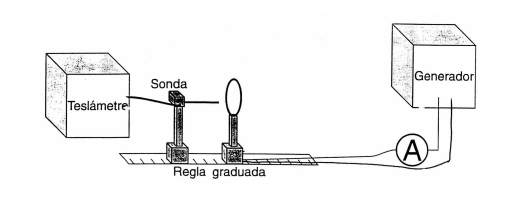
\includegraphics{circuit-teslametre.png}
  \caption{Esquema del circuit emprat per a mesurar el camp a l'eix d'una espira}
  \label{fig:circuit teslametre}
\end{figure}

El propòsit del circuit de la \cref{fig:circuit teslametre} és evidentment mesurar el camp al centre de l'espira. L'amperímetre ens resulta útil per obtenir una mesura més precisa que la donada pel generador de la intensitat que circula pel circuit. El teslàmetre indica el camp magnètic mesurat aproximadament a la punta de la sonda. Tanmateix, l'efectivitat del teslàmetre no és immediata i ha estat necessari esperar uns minuts perquè s'estabilitzi.

En concloure l'estabilització del teslàmetre, amb l'amperímetre marcant \SI{4.00}{A}, s'han pres mesures del camp col·locant la sonda al centre de l'espira. Concretament s'han pres 3 mesures en un sentit del corrent, tres mesures en l'altre i s'ha fet el promig per tal de compensar les fluctuacions del teslàmetre. Aquest procediment ha estat repetit per les tres espires a mesurar.

Posteriorment s'ha mesurat el camp al centre del conjunt de 1, 2 i 3 espires amb exactament el mateix procediment explicat.

El valor obtingut s'ha comparat amb l'esperat teòricament segons la fórmula obtinguda a partir de la llei de Biot i Savart,
\begin{equation}\label{eq:camp espira}
  \vec{B}=\frac{\mu_0 I N}{2 R}\vec{e}_z,
\end{equation}
On \( I \) és la intensitat que circula per a cada espira, \( N \) el nombre d'espires, \( R \) el seu radi i \( \vec{e}_z \) el vector unitari al llarg de l'eix de les espires. En la \cref{sec:espires} es presenten els resultats teòrics i experimentals d'aquest apartat, així com gràfics representant la variació del camp en funció del radi de l'espira i la variació en funció del nombre d'espires.

\subsection{Bobines}
Per la mesura del camp a l'interior de les bobines s'ha fet servir el mateix circuit que es mostra a la \cref{fig:circuit teslametre}.

Ajustant la intensitat a \data{1.00}{0.01}{A} a l'amperímetre, s'ha mesurat el camp a diversos punts a l'interior de la bobina. Per fer-ho s'ha ajustat l'alçada de la sonda de manera que aquesta quedi sobre l'eix interior de la bobina. Començant pel punt immediatament a l'exterior de la bobina s'ha fet avançar la sonda mesurant el camp cada \SI{3}{cm} (mesurats amb el regle) de manera que n'han resultat 8 mesures a diferents punts de l'eix.

Aquest mateix procediment s'ha repetit per cada bobina diferent i s'han comparat els valors amb els esperats de manera teòrica segons
\begin{equation}\label{eq:camp bobina}
  \vec{B}=\frac{\mu_0 I N}{2 L}\left(\frac{z + L/2}{\sqrt{R^2+(z+L/2)^2}} - \frac{z - L/2}{\sqrt{R^2 + (z - L/2)^2}}\right) \vec{e}_z,
\end{equation}
on \( I \) és la intensitat que circula per la bobina, \( N \) és el nombre de voltes de la bobina, \( L \) és la seva longitud, \( z \) és la posició de la sona al llarg de l'eix de la bobina ---fixant \( z = 0 \) al seu centre--- i \( \vec{e}_z \) és el vector unitari al llarg de l'eix. 

El valors teòrics i experimentals d'aquest apartat es presenten en la \cref{sec:bobines}.

\section{Resultats}
\subsection{Espires}\label{sec:espires}
Com s'ha mencionat anteriorment, en aquesta secció es presenten els resultats relatius a la part de la pràctica referent a les espires. A la \cref{tab:camp espires en funcio de r} es presenten les mesures del camp magnètic al centre d'una espira en funció del seu radi. 

\begin{table}[htb]
  \centering \small \sffamily
  \caption{Taula de valors teòrics i experimentals}
  \label{tab:camp espires en funcio de r}
	\begin{tabular}{SSS}
		\toprule
		{Radi (\data{}{0.2}{cm})} & { \( B_{\textsf{exp}}\ (\SI{d-5}{T}) \) } & { \( B_{\textsf{teò}}\ (\SI{d-5}{T}) \) } \\
		\midrule
		3.0 & 7.3\pm1.4 & 8.4\pm0.4 \\
		4.3 & 6.0\pm1.6 & 5.9\pm0.2 \\
		6.0 & 5.0\pm1.6 & 4.2\pm0.1 \\
		\bottomrule
	\end{tabular}
\end{table}

Les incerteses dels camps experimentals de la \cref{tab:camp espires en funcio de r} han estat calculades segons la desviació estàndard de les diferents mesures realitzades. Pel que fa a les incerteses teòriques, aquestes han estat calculades per propagació d'incerteses de la fórmula \cref{eq:camp espira}. Com podem veure en els tres casos, els valors experimentals amb els seus respectius intervals d'incertesa coincideixen en alguns punts amb els valors teòrics i els seus intervals, per tant els resultats són compatibles. Es pot observar que l'incertesa dels resultats experimentals és considerablement major. Això és degut a les imprecisions dels aparells emprats per a la mesura dels camps, especialment a les contínues fluctuacions del teslàmetre. 

Tanmateix, el fet més rellevant que podem observar és la disminució del camp a l'interior de l'espira a mesura que augmenta el seu radi. Aquest resultat ja era el que esperavem teòricament. Per fer més èmfasi en aquest fet es presenta la gràfica de lacref{fig:camp espira}, on es representa el camp magnètic al centre en funció del radi de l'espira.
\begin{figure}[htb]
  \centering
  % 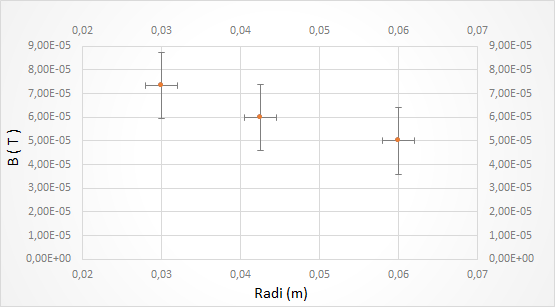
\includegraphics[width=100mm]{graf1.png}
  \caption{Camp magnètic al centre en funció del radi de l'espira}
  \label{fig:camp espira}
\end{figure}

Com es comentava, s'observa que el camp a l'interior es va  atenuant a mesura que s'augmenta el radi de l'espira. Tot i que és difícil d'apreciar ja que només s'ha fet la mesura amb tres radis diferents, es pot comprovar numèricament que el camp magnètic decau com \( \frac{1}{R} \). Aquesta és per tant la forma de funció que observaríem si es tinguessin valors infinits de radis d'espires i els seus camps respectius.

La taula \cref{tab:camp espires en funcio de n} presenta els camp magnètics teòrics i experimentals al centre dels conjunts de 1, 2 i 3 espires. 

\begin{table}[htb]
	\centering \small \sffamily
	\caption{Valors teòrics i experimentals del camp magnètic al centre d'un conjunt de \( N \) espires}
	\label{tab:camp espires en funcio de n}
	\begin{tabular}{SSS}
		\toprule
		{Nombre d'espires \( N \)} & { \( B_{\textsf{exp}}\ (\SI{d-5}{T}) \) } & { \( B_{\textsf{teò}}\ (\SI{d-5}{T}) \) } \\
		\midrule
		1 & 5.0\pm1.6 & 4.2\pm0.1 \\
		2 & 8.8\pm1.5 & 8.4\pm0.2 \\
		3 & 12.3\pm1.5 & 12.6\pm0.3 \\
		\bottomrule
	\end{tabular}
\end{table}

Podem observar que en aquest cas els intervals dels camps teòrics i experimentals també se solapen i per tant les observacions satisfan l'esperat. Altra vegada tornem a tenir incerteses majors pels valors experimentals pel mateix fet anteriorment mencionat. Els resultats ens permeten observar que com més espires introduïm al conjunt més intens es torna el camp al centre d'aquest. Aquesta dependència es pot observar clarament al gràfic experimental del camp al centre en funció del nombre d'espires que s'exposa a la \cref{fig:camp vs n}.

\begin{figure}[htb]
  \centering
  % 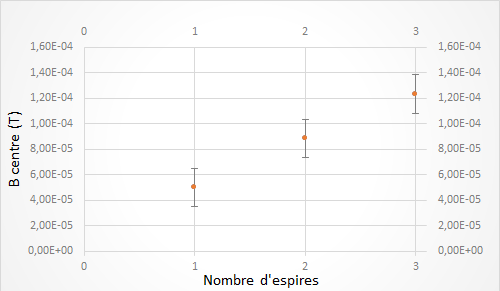
\includegraphics[width=100mm]{graf2.png}
  \caption{Camp al centre en funció del nombre d'espires}
  \label{fig:camp vs n}
\end{figure}

Podem veure a la regressió de la \cref{fig:camp vs n} que aquesta dependència és lineal com s'esperava dels valors teòrics obtinguts a partir de la \cref{eq:camp espira}. El valor de $\mu_{0}$ obtingut a partir de la regressió tenint en compte que el pendent segons \cref{eq:camp espira} és $\frac{\mu_{0}I}{2R}$  s'obté un valor de $\mu_{0} = \data{1.10}{0.37d-6}{N.A^{-2}} $ que és compatible amb el valor teòric de $\mu_{0}\approx \SI{1.26d-6}{N.A^{-2}} $. Així doncs, vist que el camp augmenta de manera directament proporcional al nombre d'espires, els resultats d'aquest apartat queden interpretats.

\subsection{Bobines}\label{sec:bobines}
\begin{figure}[tp]
	\sffamily \small
	\centering
	% GNUPLOT: LaTeX picture with Postscript
\begingroup
\sffamily \small
  \makeatletter
  \providecommand\color[2][]{%
    \GenericError{(gnuplot) \space\space\space\@spaces}{%
      Package color not loaded in conjunction with
      terminal option `colourtext'%
    }{See the gnuplot documentation for explanation.%
    }{Either use 'blacktext' in gnuplot or load the package
      color.sty in LaTeX.}%
    \renewcommand\color[2][]{}%
  }%
  \providecommand\includegraphics[2][]{%
    \GenericError{(gnuplot) \space\space\space\@spaces}{%
      Package graphicx or graphics not loaded%
    }{See the gnuplot documentation for explanation.%
    }{The gnuplot epslatex terminal needs graphicx.sty or graphics.sty.}%
    \renewcommand\includegraphics[2][]{}%
  }%
  \providecommand\rotatebox[2]{#2}%
  \@ifundefined{ifGPcolor}{%
    \newif\ifGPcolor
    \GPcolortrue
  }{}%
  \@ifundefined{ifGPblacktext}{%
    \newif\ifGPblacktext
    \GPblacktextfalse
  }{}%
  % define a \g@addto@macro without @ in the name:
  \let\gplgaddtomacro\g@addto@macro
  % define empty templates for all commands taking text:
  \gdef\gplbacktext{}%
  \gdef\gplfronttext{}%
  \makeatother
  \ifGPblacktext
    % no textcolor at all
    \def\colorrgb#1{}%
    \def\colorgray#1{}%
  \else
    % gray or color?
    \ifGPcolor
      \def\colorrgb#1{\color[rgb]{#1}}%
      \def\colorgray#1{\color[gray]{#1}}%
      \expandafter\def\csname LTw\endcsname{\color{white}}%
      \expandafter\def\csname LTb\endcsname{\color{black}}%
      \expandafter\def\csname LTa\endcsname{\color{black}}%
      \expandafter\def\csname LT0\endcsname{\color[rgb]{1,0,0}}%
      \expandafter\def\csname LT1\endcsname{\color[rgb]{0,1,0}}%
      \expandafter\def\csname LT2\endcsname{\color[rgb]{0,0,1}}%
      \expandafter\def\csname LT3\endcsname{\color[rgb]{1,0,1}}%
      \expandafter\def\csname LT4\endcsname{\color[rgb]{0,1,1}}%
      \expandafter\def\csname LT5\endcsname{\color[rgb]{1,1,0}}%
      \expandafter\def\csname LT6\endcsname{\color[rgb]{0,0,0}}%
      \expandafter\def\csname LT7\endcsname{\color[rgb]{1,0.3,0}}%
      \expandafter\def\csname LT8\endcsname{\color[rgb]{0.5,0.5,0.5}}%
    \else
      % gray
      \def\colorrgb#1{\color{black}}%
      \def\colorgray#1{\color[gray]{#1}}%
      \expandafter\def\csname LTw\endcsname{\color{white}}%
      \expandafter\def\csname LTb\endcsname{\color{black}}%
      \expandafter\def\csname LTa\endcsname{\color{black}}%
      \expandafter\def\csname LT0\endcsname{\color{black}}%
      \expandafter\def\csname LT1\endcsname{\color{black}}%
      \expandafter\def\csname LT2\endcsname{\color{black}}%
      \expandafter\def\csname LT3\endcsname{\color{black}}%
      \expandafter\def\csname LT4\endcsname{\color{black}}%
      \expandafter\def\csname LT5\endcsname{\color{black}}%
      \expandafter\def\csname LT6\endcsname{\color{black}}%
      \expandafter\def\csname LT7\endcsname{\color{black}}%
      \expandafter\def\csname LT8\endcsname{\color{black}}%
    \fi
  \fi
    \setlength{\unitlength}{0.0500bp}%
    \ifx\gptboxheight\undefined%
      \newlength{\gptboxheight}%
      \newlength{\gptboxwidth}%
      \newsavebox{\gptboxtext}%
    \fi%
    \setlength{\fboxrule}{0.5pt}%
    \setlength{\fboxsep}{1pt}%
\begin{picture}(5668.00,3400.00)%
    \gplgaddtomacro\gplbacktext{%
      \csname LTb\endcsname%%
      \put(946,704){\makebox(0,0)[r]{\strut{}\num{0}}}%
      \put(946,1117){\makebox(0,0)[r]{\strut{}\num{0.5}}}%
      \put(946,1529){\makebox(0,0)[r]{\strut{}\num{1}}}%
      \put(946,1942){\makebox(0,0)[r]{\strut{}\num{1.5}}}%
      \put(946,2354){\makebox(0,0)[r]{\strut{}\num{2}}}%
      \put(946,2767){\makebox(0,0)[r]{\strut{}\num{2.5}}}%
      \put(946,3179){\makebox(0,0)[r]{\strut{}\num{3}}}%
      \put(1078,484){\makebox(0,0){\strut{}\num{-15}}}%
      \put(1777,484){\makebox(0,0){\strut{}\num{-10}}}%
      \put(2476,484){\makebox(0,0){\strut{}\num{-5}}}%
      \put(3175,484){\makebox(0,0){\strut{}\num{0}}}%
      \put(3873,484){\makebox(0,0){\strut{}\num{5}}}%
      \put(4572,484){\makebox(0,0){\strut{}\num{10}}}%
      \put(5271,484){\makebox(0,0){\strut{}\num{15}}}%
    }%
    \gplgaddtomacro\gplfronttext{%
      \csname LTb\endcsname%%
      \put(198,1941){\rotatebox{-270}{\makebox(0,0){\strut{}$\mathsf{B \ (\si{mT})}$}}}%
      \put(3174,154){\makebox(0,0){\strut{}$\mathsf{z \ (\si{cm})}$}}%
    }%
    \gplbacktext
    \put(0,0){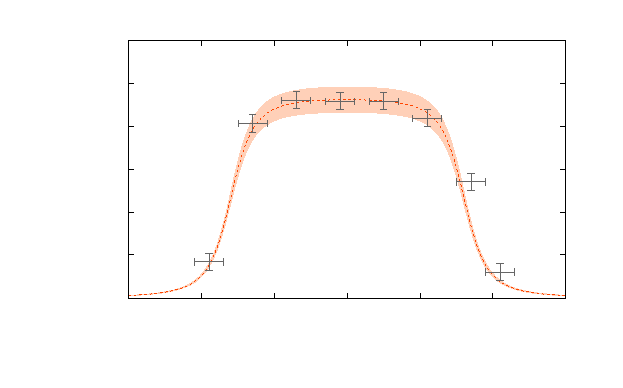
\includegraphics{camp-300-33}}%
    \gplfronttext
  \end{picture}%
\endgroup

	\caption{Camp magnètic al llarg de l'eix d'una bobina de 300 voltes, longitud \SI{16}{cm} i diàmetre \SI{3.3}{cm} per la que hi passa un corrent constant de \SI{1}{A}.}
	\label{fig:camp 300/33}
\end{figure}

\begin{figure}[tp]
	\sffamily \small
	\centering
	% GNUPLOT: LaTeX picture with Postscript
\begingroup
\sffamily \small
  \makeatletter
  \providecommand\color[2][]{%
    \GenericError{(gnuplot) \space\space\space\@spaces}{%
      Package color not loaded in conjunction with
      terminal option `colourtext'%
    }{See the gnuplot documentation for explanation.%
    }{Either use 'blacktext' in gnuplot or load the package
      color.sty in LaTeX.}%
    \renewcommand\color[2][]{}%
  }%
  \providecommand\includegraphics[2][]{%
    \GenericError{(gnuplot) \space\space\space\@spaces}{%
      Package graphicx or graphics not loaded%
    }{See the gnuplot documentation for explanation.%
    }{The gnuplot epslatex terminal needs graphicx.sty or graphics.sty.}%
    \renewcommand\includegraphics[2][]{}%
  }%
  \providecommand\rotatebox[2]{#2}%
  \@ifundefined{ifGPcolor}{%
    \newif\ifGPcolor
    \GPcolortrue
  }{}%
  \@ifundefined{ifGPblacktext}{%
    \newif\ifGPblacktext
    \GPblacktextfalse
  }{}%
  % define a \g@addto@macro without @ in the name:
  \let\gplgaddtomacro\g@addto@macro
  % define empty templates for all commands taking text:
  \gdef\gplbacktext{}%
  \gdef\gplfronttext{}%
  \makeatother
  \ifGPblacktext
    % no textcolor at all
    \def\colorrgb#1{}%
    \def\colorgray#1{}%
  \else
    % gray or color?
    \ifGPcolor
      \def\colorrgb#1{\color[rgb]{#1}}%
      \def\colorgray#1{\color[gray]{#1}}%
      \expandafter\def\csname LTw\endcsname{\color{white}}%
      \expandafter\def\csname LTb\endcsname{\color{black}}%
      \expandafter\def\csname LTa\endcsname{\color{black}}%
      \expandafter\def\csname LT0\endcsname{\color[rgb]{1,0,0}}%
      \expandafter\def\csname LT1\endcsname{\color[rgb]{0,1,0}}%
      \expandafter\def\csname LT2\endcsname{\color[rgb]{0,0,1}}%
      \expandafter\def\csname LT3\endcsname{\color[rgb]{1,0,1}}%
      \expandafter\def\csname LT4\endcsname{\color[rgb]{0,1,1}}%
      \expandafter\def\csname LT5\endcsname{\color[rgb]{1,1,0}}%
      \expandafter\def\csname LT6\endcsname{\color[rgb]{0,0,0}}%
      \expandafter\def\csname LT7\endcsname{\color[rgb]{1,0.3,0}}%
      \expandafter\def\csname LT8\endcsname{\color[rgb]{0.5,0.5,0.5}}%
    \else
      % gray
      \def\colorrgb#1{\color{black}}%
      \def\colorgray#1{\color[gray]{#1}}%
      \expandafter\def\csname LTw\endcsname{\color{white}}%
      \expandafter\def\csname LTb\endcsname{\color{black}}%
      \expandafter\def\csname LTa\endcsname{\color{black}}%
      \expandafter\def\csname LT0\endcsname{\color{black}}%
      \expandafter\def\csname LT1\endcsname{\color{black}}%
      \expandafter\def\csname LT2\endcsname{\color{black}}%
      \expandafter\def\csname LT3\endcsname{\color{black}}%
      \expandafter\def\csname LT4\endcsname{\color{black}}%
      \expandafter\def\csname LT5\endcsname{\color{black}}%
      \expandafter\def\csname LT6\endcsname{\color{black}}%
      \expandafter\def\csname LT7\endcsname{\color{black}}%
      \expandafter\def\csname LT8\endcsname{\color{black}}%
    \fi
  \fi
    \setlength{\unitlength}{0.0500bp}%
    \ifx\gptboxheight\undefined%
      \newlength{\gptboxheight}%
      \newlength{\gptboxwidth}%
      \newsavebox{\gptboxtext}%
    \fi%
    \setlength{\fboxrule}{0.5pt}%
    \setlength{\fboxsep}{1pt}%
\begin{picture}(5668.00,3400.00)%
    \gplgaddtomacro\gplbacktext{%
      \csname LTb\endcsname%%
      \put(946,704){\makebox(0,0)[r]{\strut{}\num{0}}}%
      \put(946,1199){\makebox(0,0)[r]{\strut{}\num{0.2}}}%
      \put(946,1694){\makebox(0,0)[r]{\strut{}\num{0.4}}}%
      \put(946,2189){\makebox(0,0)[r]{\strut{}\num{0.6}}}%
      \put(946,2684){\makebox(0,0)[r]{\strut{}\num{0.8}}}%
      \put(946,3179){\makebox(0,0)[r]{\strut{}\num{1}}}%
      \put(1078,484){\makebox(0,0){\strut{}\num{-15}}}%
      \put(1777,484){\makebox(0,0){\strut{}\num{-10}}}%
      \put(2476,484){\makebox(0,0){\strut{}\num{-5}}}%
      \put(3175,484){\makebox(0,0){\strut{}\num{0}}}%
      \put(3873,484){\makebox(0,0){\strut{}\num{5}}}%
      \put(4572,484){\makebox(0,0){\strut{}\num{10}}}%
      \put(5271,484){\makebox(0,0){\strut{}\num{15}}}%
    }%
    \gplgaddtomacro\gplfronttext{%
      \csname LTb\endcsname%%
      \put(198,1941){\rotatebox{-270}{\makebox(0,0){\strut{}$\mathsf{B \ (\si{mT})}$}}}%
      \put(3174,154){\makebox(0,0){\strut{}$\mathsf{z \ (\si{cm})}$}}%
    }%
    \gplbacktext
    \put(0,0){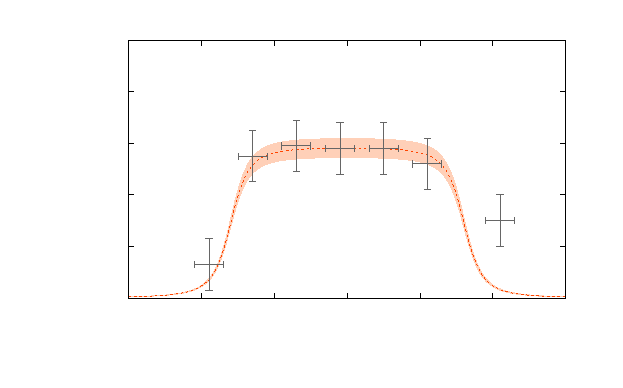
\includegraphics{camp-75-26}}%
    \gplfronttext
  \end{picture}%
\endgroup

	\caption{Camp magnètic al llarg de l'eix d'una bobina de 75 voltes, longitud \SI{16}{cm} i diàmetre \SI{2.6}{cm} per la que hi passa un corrent constant de \SI{1}{A}.}
	\label{fig:camp 75/26}
\end{figure}

\begin{figure}[tp]
	\sffamily \small
	\centering
	% GNUPLOT: LaTeX picture with Postscript
\begingroup
\sffamily \small
  \makeatletter
  \providecommand\color[2][]{%
    \GenericError{(gnuplot) \space\space\space\@spaces}{%
      Package color not loaded in conjunction with
      terminal option `colourtext'%
    }{See the gnuplot documentation for explanation.%
    }{Either use 'blacktext' in gnuplot or load the package
      color.sty in LaTeX.}%
    \renewcommand\color[2][]{}%
  }%
  \providecommand\includegraphics[2][]{%
    \GenericError{(gnuplot) \space\space\space\@spaces}{%
      Package graphicx or graphics not loaded%
    }{See the gnuplot documentation for explanation.%
    }{The gnuplot epslatex terminal needs graphicx.sty or graphics.sty.}%
    \renewcommand\includegraphics[2][]{}%
  }%
  \providecommand\rotatebox[2]{#2}%
  \@ifundefined{ifGPcolor}{%
    \newif\ifGPcolor
    \GPcolortrue
  }{}%
  \@ifundefined{ifGPblacktext}{%
    \newif\ifGPblacktext
    \GPblacktextfalse
  }{}%
  % define a \g@addto@macro without @ in the name:
  \let\gplgaddtomacro\g@addto@macro
  % define empty templates for all commands taking text:
  \gdef\gplbacktext{}%
  \gdef\gplfronttext{}%
  \makeatother
  \ifGPblacktext
    % no textcolor at all
    \def\colorrgb#1{}%
    \def\colorgray#1{}%
  \else
    % gray or color?
    \ifGPcolor
      \def\colorrgb#1{\color[rgb]{#1}}%
      \def\colorgray#1{\color[gray]{#1}}%
      \expandafter\def\csname LTw\endcsname{\color{white}}%
      \expandafter\def\csname LTb\endcsname{\color{black}}%
      \expandafter\def\csname LTa\endcsname{\color{black}}%
      \expandafter\def\csname LT0\endcsname{\color[rgb]{1,0,0}}%
      \expandafter\def\csname LT1\endcsname{\color[rgb]{0,1,0}}%
      \expandafter\def\csname LT2\endcsname{\color[rgb]{0,0,1}}%
      \expandafter\def\csname LT3\endcsname{\color[rgb]{1,0,1}}%
      \expandafter\def\csname LT4\endcsname{\color[rgb]{0,1,1}}%
      \expandafter\def\csname LT5\endcsname{\color[rgb]{1,1,0}}%
      \expandafter\def\csname LT6\endcsname{\color[rgb]{0,0,0}}%
      \expandafter\def\csname LT7\endcsname{\color[rgb]{1,0.3,0}}%
      \expandafter\def\csname LT8\endcsname{\color[rgb]{0.5,0.5,0.5}}%
    \else
      % gray
      \def\colorrgb#1{\color{black}}%
      \def\colorgray#1{\color[gray]{#1}}%
      \expandafter\def\csname LTw\endcsname{\color{white}}%
      \expandafter\def\csname LTb\endcsname{\color{black}}%
      \expandafter\def\csname LTa\endcsname{\color{black}}%
      \expandafter\def\csname LT0\endcsname{\color{black}}%
      \expandafter\def\csname LT1\endcsname{\color{black}}%
      \expandafter\def\csname LT2\endcsname{\color{black}}%
      \expandafter\def\csname LT3\endcsname{\color{black}}%
      \expandafter\def\csname LT4\endcsname{\color{black}}%
      \expandafter\def\csname LT5\endcsname{\color{black}}%
      \expandafter\def\csname LT6\endcsname{\color{black}}%
      \expandafter\def\csname LT7\endcsname{\color{black}}%
      \expandafter\def\csname LT8\endcsname{\color{black}}%
    \fi
  \fi
    \setlength{\unitlength}{0.0500bp}%
    \ifx\gptboxheight\undefined%
      \newlength{\gptboxheight}%
      \newlength{\gptboxwidth}%
      \newsavebox{\gptboxtext}%
    \fi%
    \setlength{\fboxrule}{0.5pt}%
    \setlength{\fboxsep}{1pt}%
\begin{picture}(5668.00,3400.00)%
    \gplgaddtomacro\gplbacktext{%
      \csname LTb\endcsname%%
      \put(946,704){\makebox(0,0)[r]{\strut{}\num{0}}}%
      \put(946,1323){\makebox(0,0)[r]{\strut{}\num{0.5}}}%
      \put(946,1942){\makebox(0,0)[r]{\strut{}\num{1}}}%
      \put(946,2560){\makebox(0,0)[r]{\strut{}\num{1.5}}}%
      \put(946,3179){\makebox(0,0)[r]{\strut{}\num{2}}}%
      \put(1078,484){\makebox(0,0){\strut{}\num{-15}}}%
      \put(1777,484){\makebox(0,0){\strut{}\num{-10}}}%
      \put(2476,484){\makebox(0,0){\strut{}\num{-5}}}%
      \put(3175,484){\makebox(0,0){\strut{}\num{0}}}%
      \put(3873,484){\makebox(0,0){\strut{}\num{5}}}%
      \put(4572,484){\makebox(0,0){\strut{}\num{10}}}%
      \put(5271,484){\makebox(0,0){\strut{}\num{15}}}%
    }%
    \gplgaddtomacro\gplfronttext{%
      \csname LTb\endcsname%%
      \put(198,1941){\rotatebox{-270}{\makebox(0,0){\strut{}$\mathsf{B \ (\si{mT})}$}}}%
      \put(3174,154){\makebox(0,0){\strut{}$\mathsf{z \ (\si{cm})}$}}%
    }%
    \gplbacktext
    \put(0,0){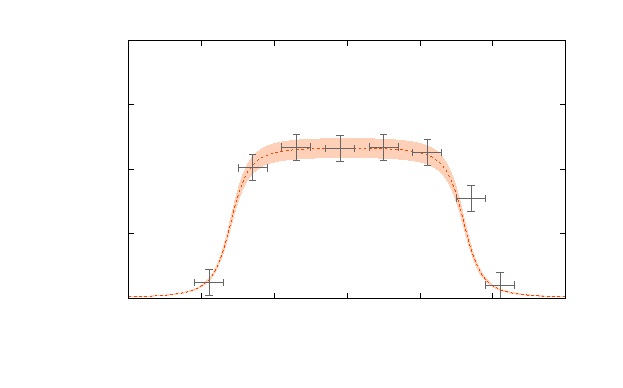
\includegraphics{camp-150-26}}%
    \gplfronttext
  \end{picture}%
\endgroup

	\caption{Camp magnètic al llarg de l'eix d'una bobina de 150 voltes, longitud \SI{16}{cm} i diàmetre \SI{2.6}{cm} per la que hi passa un corrent constant de \SI{1}{A}.}
	\label{fig:camp 150/26}
\end{figure}

\begin{figure}[tp]
	\sffamily \small
	\centering
	% GNUPLOT: LaTeX picture with Postscript
\begingroup
\sffamily \small
  \makeatletter
  \providecommand\color[2][]{%
    \GenericError{(gnuplot) \space\space\space\@spaces}{%
      Package color not loaded in conjunction with
      terminal option `colourtext'%
    }{See the gnuplot documentation for explanation.%
    }{Either use 'blacktext' in gnuplot or load the package
      color.sty in LaTeX.}%
    \renewcommand\color[2][]{}%
  }%
  \providecommand\includegraphics[2][]{%
    \GenericError{(gnuplot) \space\space\space\@spaces}{%
      Package graphicx or graphics not loaded%
    }{See the gnuplot documentation for explanation.%
    }{The gnuplot epslatex terminal needs graphicx.sty or graphics.sty.}%
    \renewcommand\includegraphics[2][]{}%
  }%
  \providecommand\rotatebox[2]{#2}%
  \@ifundefined{ifGPcolor}{%
    \newif\ifGPcolor
    \GPcolortrue
  }{}%
  \@ifundefined{ifGPblacktext}{%
    \newif\ifGPblacktext
    \GPblacktextfalse
  }{}%
  % define a \g@addto@macro without @ in the name:
  \let\gplgaddtomacro\g@addto@macro
  % define empty templates for all commands taking text:
  \gdef\gplbacktext{}%
  \gdef\gplfronttext{}%
  \makeatother
  \ifGPblacktext
    % no textcolor at all
    \def\colorrgb#1{}%
    \def\colorgray#1{}%
  \else
    % gray or color?
    \ifGPcolor
      \def\colorrgb#1{\color[rgb]{#1}}%
      \def\colorgray#1{\color[gray]{#1}}%
      \expandafter\def\csname LTw\endcsname{\color{white}}%
      \expandafter\def\csname LTb\endcsname{\color{black}}%
      \expandafter\def\csname LTa\endcsname{\color{black}}%
      \expandafter\def\csname LT0\endcsname{\color[rgb]{1,0,0}}%
      \expandafter\def\csname LT1\endcsname{\color[rgb]{0,1,0}}%
      \expandafter\def\csname LT2\endcsname{\color[rgb]{0,0,1}}%
      \expandafter\def\csname LT3\endcsname{\color[rgb]{1,0,1}}%
      \expandafter\def\csname LT4\endcsname{\color[rgb]{0,1,1}}%
      \expandafter\def\csname LT5\endcsname{\color[rgb]{1,1,0}}%
      \expandafter\def\csname LT6\endcsname{\color[rgb]{0,0,0}}%
      \expandafter\def\csname LT7\endcsname{\color[rgb]{1,0.3,0}}%
      \expandafter\def\csname LT8\endcsname{\color[rgb]{0.5,0.5,0.5}}%
    \else
      % gray
      \def\colorrgb#1{\color{black}}%
      \def\colorgray#1{\color[gray]{#1}}%
      \expandafter\def\csname LTw\endcsname{\color{white}}%
      \expandafter\def\csname LTb\endcsname{\color{black}}%
      \expandafter\def\csname LTa\endcsname{\color{black}}%
      \expandafter\def\csname LT0\endcsname{\color{black}}%
      \expandafter\def\csname LT1\endcsname{\color{black}}%
      \expandafter\def\csname LT2\endcsname{\color{black}}%
      \expandafter\def\csname LT3\endcsname{\color{black}}%
      \expandafter\def\csname LT4\endcsname{\color{black}}%
      \expandafter\def\csname LT5\endcsname{\color{black}}%
      \expandafter\def\csname LT6\endcsname{\color{black}}%
      \expandafter\def\csname LT7\endcsname{\color{black}}%
      \expandafter\def\csname LT8\endcsname{\color{black}}%
    \fi
  \fi
    \setlength{\unitlength}{0.0500bp}%
    \ifx\gptboxheight\undefined%
      \newlength{\gptboxheight}%
      \newlength{\gptboxwidth}%
      \newsavebox{\gptboxtext}%
    \fi%
    \setlength{\fboxrule}{0.5pt}%
    \setlength{\fboxsep}{1pt}%
\begin{picture}(5668.00,3400.00)%
    \gplgaddtomacro\gplbacktext{%
      \csname LTb\endcsname%%
      \put(946,704){\makebox(0,0)[r]{\strut{}\num{0}}}%
      \put(946,1013){\makebox(0,0)[r]{\strut{}\num{0.5}}}%
      \put(946,1323){\makebox(0,0)[r]{\strut{}\num{1}}}%
      \put(946,1632){\makebox(0,0)[r]{\strut{}\num{1.5}}}%
      \put(946,1942){\makebox(0,0)[r]{\strut{}\num{2}}}%
      \put(946,2251){\makebox(0,0)[r]{\strut{}\num{2.5}}}%
      \put(946,2560){\makebox(0,0)[r]{\strut{}\num{3}}}%
      \put(946,2870){\makebox(0,0)[r]{\strut{}\num{3.5}}}%
      \put(946,3179){\makebox(0,0)[r]{\strut{}\num{4}}}%
      \put(1078,484){\makebox(0,0){\strut{}\num{-15}}}%
      \put(1777,484){\makebox(0,0){\strut{}\num{-10}}}%
      \put(2476,484){\makebox(0,0){\strut{}\num{-5}}}%
      \put(3175,484){\makebox(0,0){\strut{}\num{0}}}%
      \put(3873,484){\makebox(0,0){\strut{}\num{5}}}%
      \put(4572,484){\makebox(0,0){\strut{}\num{10}}}%
      \put(5271,484){\makebox(0,0){\strut{}\num{15}}}%
    }%
    \gplgaddtomacro\gplfronttext{%
      \csname LTb\endcsname%%
      \put(198,1941){\rotatebox{-270}{\makebox(0,0){\strut{}$\mathsf{B \ (\si{mT})}$}}}%
      \put(3174,154){\makebox(0,0){\strut{}$\mathsf{z \ (\si{cm})}$}}%
    }%
    \gplbacktext
    \put(0,0){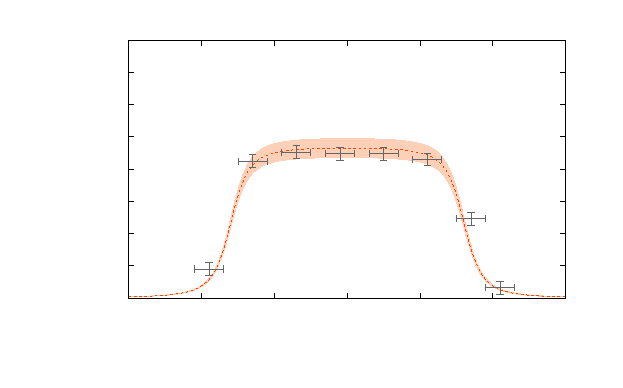
\includegraphics{camp-300-26}}%
    \gplfronttext
  \end{picture}%
\endgroup

	\caption{Camp magnètic al llarg de l'eix d'una bobina de 300 voltes, longitud \SI{16}{cm} i diàmetre \SI{2.6}{cm} per la que hi passa un corrent constant de \SI{1}{A}.}
	\label{fig:camp 300/26}
\end{figure}

A les \cref{fig:camp 300/33,fig:camp 75/26,fig:camp 150/26,fig:camp 300/26} hi ha representat el mòdul del camp magnètic al llarg de l'eix de les bobines mesurades durant l'experiment---calculat a partir de l'\cref{eq:camp bobina} i amb el corresponent marge d'incertesa--- aixì com els punts corresponents a les mesures realitzades

Tal i com es pot apreciar, al llarg de l'eix les mesures obtingudes s'ajusten molt bé a la prediccío teòrica. Això és d'esperar ja que a l'interior d'una bobina el camp és pràcticament constant. Als extrems, però, les dades experimentals no s'hi ajusten tant. Una explicació és que en  

\section{Conclusions}
En general els resultats obtinguts han estat satisfactoris. S'ha observat empíricament al llarg de tota la pràctica els fets que s'havien demostrat de manera teòrica. El camp magnètic al centre d'una espira disminueix a mesura que augmenta el radi d'aquesta i ho fa com $\frac{1}{R}$ amb $R$ el radi de l'espira. S'ha comprovat també empíricament l'augment lineal del camp al centre d'un conjunt d'espires amb la quantitat d'espires. Aquest últim fet ha estat provat per conjunts de $1$, $2$ i $3$ espires. Les observacions han portat també a concloure que el camp magnètic al centre d'una bobina augmenta en apropar-se al centre i és màxim en aquest. El fet que el camp magnètic creat per una bobina on hi circula una certa intensitat augmenta amb el nombre de voltes, ha estat provat també de manera satisfactòria. Finalment s'ha calculat empíricament la permeabilitat magnètica $\mu_{0}$ i s'ha obtingut una bona aproximació d'aquesta.




